\documentclass[a4paper,10pt]{article}
\usepackage[margin=1in]{geometry}
\usepackage{polski}
\usepackage[utf8x]{inputenc}
\usepackage[unicode]{hyperref}
\usepackage{amssymb}
\usepackage{xifthen}
\usepackage[fleqn]{amsmath}
\usepackage{todonotes}
\usepackage{graphicx}
\usepackage{float}
\usepackage{fullpage}
\usepackage{epstopdf}
\usepackage{multirow}
\usepackage{subfig}
\usepackage{booktabs}
\usepackage[europeanresistors,americaninductors]{circuitikz}
\usetikzlibrary{patterns}
\newcommand{\withtodo}{0}

\def\arraystretch{1.2}

\begin{document}

\begin{table}
  \centering
  \def\arraystretch{1.5}
    \begin{tabular}{|l|l|l|l|} \hline
    Wydział:           & \multicolumn{2}{l|}{Dzień:Poniedziałek 14-17}    &Zespół:  \\
    Fizyki             &    \multicolumn{2}{l|}{Data: 20.03.2017}         &8             \\\hline
    Imiona i nazwiska: &Ocena z przygotowania:  &Ocena ze sprawozdania:   &Ocena końcowa: \\
    Marta Pogorzelska  &                        &                         &                \\
    Paulina Marikin    &                        &                         &\\\hline
    \multicolumn{2}{|l|}{Prowadzący:                 } &\multicolumn{2}{l|}{Podpis:             }  \\\hline
  \end{tabular}
\end{table}


\title{Ćwiczenie 3:\\Wahadło matematyczne}
\date{}
\maketitle{}

\section{Cel badań}
Zbadanie zjawiska anharmoniczności drgań wahadła matematycznego, tj: zależności okresu drgań wahadła od kąta wychylenia oraz wyznaczenie wartości przyspieszenia ziemskiego przy użyciu wahadła różnicowego.

\section{Wstęp teoretyczny}
Wahadłem matematycznym jest ciało o masie punktowej m, zawieszone na cienkiej, nieważkiej lince, poruszające się po okręgu w jednorodnym polu grawitacyjnym.
\\
\\
\\
\begin{figure}[H]
\centering
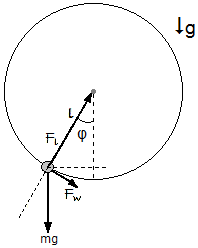
\includegraphics[width=0.3\textwidth]{wahadlo.png}
\caption{Wahadło matematyczne \\$F_w$ - siła wypadkowa działająca na ciało}
\end{figure}.
\\
\\Na ciało działa siła grawitacji oraz siła naciągu linki. Równanie ruchu dla takiego ciała ma postać:
\begin{equation}
\frac{d^2\varphi}{dt^2} + \frac{g}{l}\sin\varphi = 0
\end{equation}
,gdzie $\varphi$ - kąt wychylenia wahadła z pozycji równowagi, l - długość linki, g - przyspieszenie ziemskie
\\
\\Rozwiązaniem tego równania dla ruchu oscylującego i jednocześnie wzorem na okres drgań wahadła jest:
\begin{equation}
T(\varphi) = 2\pi\sqrt{\frac{l}{g}}\sum_{n=0}^{\infty}\bigg(\frac{(2n)!}{(2^nn!)^2}\bigg)^2\sin^{2n}\bigg(\frac{\varphi}{2}\bigg)
\end{equation}

W przeprowadzanym doświadczeniu kąt wychylenia jest niewielki $\varphi<<\frac{\pi}{2}$. Dla dokładnośći 3 miejsc znaczących będą brane pod uwagę jedynie sumy dla n=3. Po podstawieniu tych zależności do wzoru (2) otrzymujemy:
\begin{equation}
T(\varphi) = 2\pi\sqrt{\frac{l}{g}}\bigg(1+\frac{1}{4}\sin^2\frac{\varphi}{2}+\frac{9}{64}\sin^4\frac{\varphi}{2}+\frac{25}{256}\sin^6\frac{\varphi}{2}\bigg)
\end{equation}

\section{Opis układu i metody pomiarowej}
Aparatura pomiarowa
\begin{itemize}
  \item model wahadła matematycznego
\begin{itemize}
  \item statyw
  \item metalowe ciało o regularnym kształcie
  \item jedwabna nić
  \item czujka do mierzenia okreu
\end{itemize}
  \item elektroniczny układ pomiarowy z automatycznym pomiarem okresu
  \item linijka
\end{itemize}
 
\subsection{Badanie zależności okresu drgań wahadła od kąta wychylenia}
Najpierw wykonano pomiar długości linki przy użyciu linijki od środka masy kulki do punktu zaczepienia  i włączono urządzenie do pomiaru okresu drgań wahadła. Nastawiono je na uśrednienie pomiaru 4 okresów. Następnie odchylono kulkę o kąt $10\,^{\circ}$ od położenia równowagi i puszczono tak, by poruszała się równolegle do kątomierza na statywie. Na koniec złapano kulkę i spisano wynik z urządzenia oraz kąt odchylenia kulki po jej złapaniu. Czynność powtórzono pięciokrotnie, a pomiary wykonano dla kątów odchylenia  $10\,^{\circ}, 20\,^{\circ}, 30\,^{\circ}$ i $40\,^{\circ}$.
\\
%\\W przeprowadzanym doświadczeniu kąt wychylenia jest nieduży ($\varphi<\frac{\pi}{2}$). Dla dokładnośći 3 miejsc znaczących wystarczy branie pod uwagę jedynie sumy dla n=3. Po podstawieniu tych zależności do wzoru (2) otrzymujemy:
%\begin{equation}
%T(\varphi) = 2\pi\sqrt{\frac{l}{g}}\bigg(1+\frac{1}{4}\sin^2\frac{\varphi}{2}+\frac{9}{64}\sin^4\frac{\varphi}{2}+\frac{25}{256}\sin^6\frac{\varphi}{2}\bigg)
%\end{equation}

\subsection{Wyznaczenie wartości przyspieszenia ziemskiego}
W tej części doświadczenia wykonane zostały pomiary okresów dla stałego kąta wychylenia, ale dla różnych długości linki wahadła. Przyjmujęto stały, mały kąt $15\,^{\circ}$ i wykonano ćwiczenie analogicznie do poprzedniego. Długość odczytano z linijki na statywie, ponieważ do obliczeń potrzebna jest jedynie zmiana w długości wahadła, a nie odległość względem pewnego punktu odniesienia. Pomiary wykonano dla odczytów 50cm, 40cm, 30cm, 20cm, 10cm i 1,5cm. Do obliczeń korzystano ze wzoru:
\begin{equation}
T_i^2-T_j^2 = \frac{4\pi^2}{g}(l_i-l_j)f(\varphi)
\end{equation}
,gdzie $f(\varphi)=\sum_{n=0}^{\infty}\bigg(\frac{(2n)!}{(2^nn!)^2}\bigg)^2\sin^{2n}\bigg(\frac{\varphi}{2}\bigg)$

\section{Wyniki pomiarów}
\subsection{Wahadło matematyczne $l=50cm$}
\begin{tabular}{lrrrr}
\toprule
{} &    $10^\circ$ &     $20^\circ$ &      $30^\circ$ &      $40^\circ$\\
\midrule
1 &  4.9223 &  5.7827 &  5.7889 &  5.8451 \\
2 &  5.6868 &  5.7221 &  5.7733 &  5.8451 \\
3 &  4.9163 &  5.7227 &  5.7745 &  5.8525 \\
4 &  5.6908 &  5.7202 &  5.7716 &  5.8456 \\
5 &  4.9222 &  5.7210 &  5.7750 &  5.8459 \\
\bottomrule
\end{tabular}
\subsection{Wahadło różnicowe\\$\varphi = 15^\circ$}
\begin{tabular}{lrrrrrr}
\toprule
{} &      50cm &      40cm &      30cm &      20cm &      10cm &     1.5cm \\
\midrule
1 &  1.2158 &  1.3703 &  1.5107 &  1.6406 &  1.7587 &  1.8516 \\
2 &  1.2122 &  1.3690 &  1.5121 &  1.6403 &  1.7599 &  1.8525 \\
3 &  1.2103 &  1.3705 &  1.5118 &  1.6403 &  1.7605 &  1.8518 \\
4 &  1.2121 &  1.3703 &  1.5124 &  1.6402 &  1.7597 &  1.8516 \\
5 &  1.2126 &  1.3706 &  1.5124 &  1.6408 &  1.7599 &  1.8518 \\
6 &  1.2136 &  1.3704 &  1.5120 &  1.6400 &  1.7605 &  1.8523 \\
\bottomrule
\end{tabular}

\section{Analiza pomiarów}
\begin{figure}[H]
    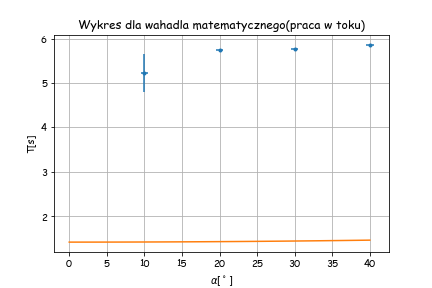
\includegraphics{./Wykres_matematyczne.png}
    \caption{}
    \label{}
\end{figure}
Z pomiarów czasu dla wszystkich serii dla obu wahadeł wyciągnięto średnią. Pomiary dla wahadła matematycznego zostały podzielone na trzy w celu uzyskania pojedyńczego okresu. Krzywą teoretyczną wyliczono ze wzoru 3. Pomiary dla trzech z czterech rozważanych kątów leżą na krzywej teoretycznej, jeden mieści ją w przedziale dwóch niepewności.
Jednak biorąc pod uwagę skalę jego niepewności, w porównaniu do pozostałych pomiarów, prawdopodobnie te pomary okresu były nieprawidłowo wykonane.
\begin{figure}[H]
    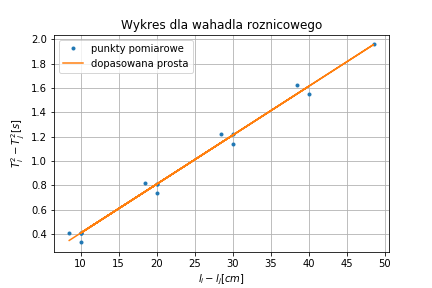
\includegraphics{./Wykres_roznicowe.png}
    \caption{}
    \label{}
\end{figure}
Pomiary zostały opracowane zgodnie ze wzorem 4, od każdego pomiaru długości (i kwadratu odpowiadającego mu pomiaru okresu) odjęto wszystkie pomiary odeń mniejsze. Otrzymane różnice przedstawiono na wykresie wraz z dopasowaną do nich prostą. Prosta zostałą dopasowana funkcją \emph{polyfit} pakietu \emph{numpy} 
w Pythonie.\\
\\
Parametr kierunkowy dopasowanej prostej został przyrównany do pozostałej części zależności 4:
\begin{equation}
a = \frac{4 \pi^2}{g} f(\varphi)
\end{equation}
gdzie a - parametr kierunkowy. Przekształcenie powyższej równości pozwoliło na wyliczenie przyspieszenia ziemskiego, którego wyliczona wartość wynosi g = 9.841(0.299)[$\frac{m}{s^2}$]
\section{Analiza niepewności}

\section{Wnioski}


\end{document}
